\chapter[Gerenciamento do Projeto]{Gerenciamento do Projeto}

\section{Termo de Abertura do Projeto}



\subsection{Estrutura Analítica do Projeto}

\begin{landscape}
	\begin{figure}
		\centering
		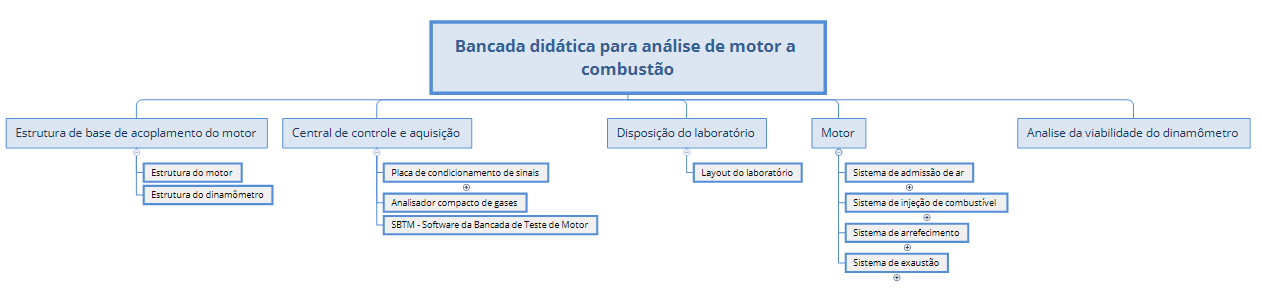
\includegraphics[keepaspectratio=true,scale= 0.8]{figuras/EAP.PNG}
		\caption{EAP}
		\label{eap}
	\end{figure}
\end{landscape}

\subsection{Cronograma}

\begin{figure}[h!]
	\centering
	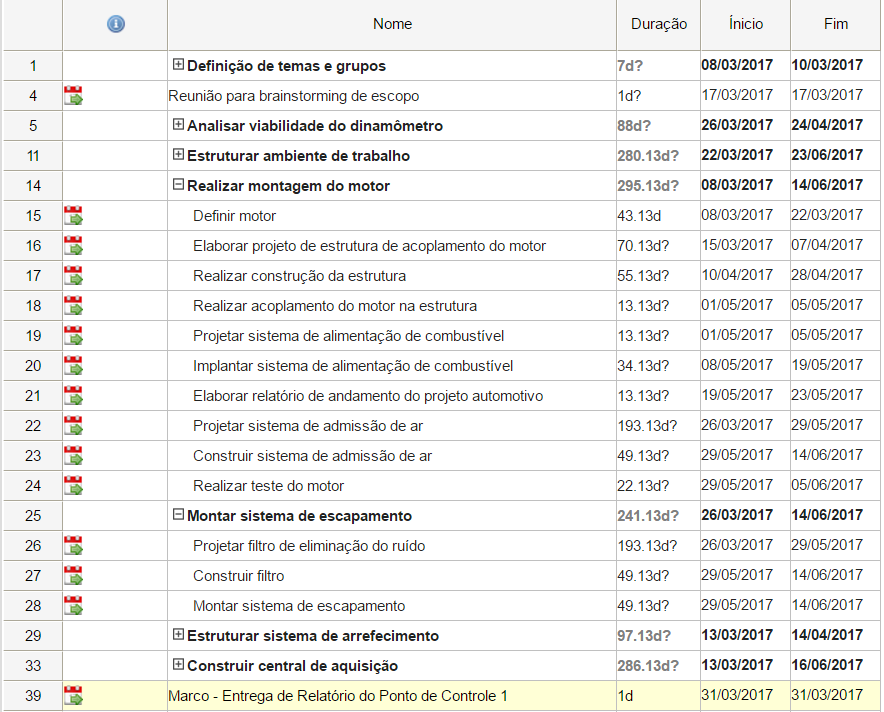
\includegraphics[keepaspectratio=true,scale= 0.8]{figuras/cronograma-PI2-parte1.PNG}
	\caption{Cronograma - Parte 1}
	\label{eap}
\end{figure}

\begin{figure}[h!]
	\centering
	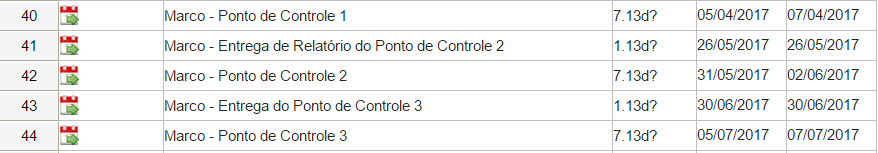
\includegraphics[keepaspectratio=true,scale= 0.8]{figuras/cronograma-PI2-parte2.PNG}
	\caption{Cronograma - Parte 2}
	\label{eap}
\end{figure}


\subsection{Custos}

\begin{table}[h!]
	\centering
	\caption{Tabela de custos geral}
	\label{tabela-custos-geral}
	\begin{tabular}{|l|l|l|l|l|}
		\hline
		\textbf{Componente}                                                                                   & \textbf{Preço(Unidade)} & \textbf{Qtd} & \textbf{Total} & \textbf{Loja: Links para consulta}                                                                                                                                                                        \\ \hline
		AD595                                                                                                 & R\$ 87,00               & 6            & R\$522,00      & \begin{tabular}[c]{@{}l@{}}http://produto.mercadolivre.com.br/\\ MLB-712124692-ad595-thermocou\\ ple-amplifier-circuito-integrado-\_\\ JM?source=gps\end{tabular}                                         \\ \hline
		\begin{tabular}[c]{@{}l@{}}Sensor De \\ Pressão Mpx5700\end{tabular}                                  & R\$ 60,00               & 6            & R\$360,00      & \begin{tabular}[c]{@{}l@{}}http://produto.mercadolivre.com.br/\\ MLB-708718648-sensor-de-presso\\ -mpx5700-para-arduino-pic-e-etc-\_\\ JM?source=gps\end{tabular}                                         \\ \hline
		\begin{tabular}[c]{@{}l@{}}Kit para Placa de\\ Circuito Impresso\end{tabular}                         & R\$ 65,00               & 1            & R\$65,00       & \begin{tabular}[c]{@{}l@{}}http://produto.mercadolivre.com.br/\\ MLB-715578391-kit-p-confecciona\\ r-placa-de-circuito-impresso-suekit\\ -ck-3-\_JM\end{tabular}                                          \\ \hline
		\begin{tabular}[c]{@{}l@{}}Placa de Circuito\\ Impresso\end{tabular}                                  & R\$ 11,39               & 2            & R\$ 22,78      & \begin{tabular}[c]{@{}l@{}}http://www.huinfinito.com.br/plac\\ as-circuito-impresso/636-placa-fe\\ nolite-virgem-face-simples-20x20\\ cm.html?search\_query=circuito+i\\ mpresso\&results=12\end{tabular} \\ \hline
		MSP430                                                                                                & R\$ 85,00               & 2            & R\$ 170,00     & \begin{tabular}[c]{@{}l@{}}2http://produto.mercadolivre.com.\\ br/MLB-842870672-microcontro\\ lador-msp430-hercules-launchpad-\\ \_JM\end{tabular}                                                        \\ \hline
		RaspBerry Pi                                                                                          & R\$ 189,98              & 1            & R\$ 189,98     & \begin{tabular}[c]{@{}l@{}}http://produto.mercadolivre.com.br\\ /MLB-810455120-novo-raspberry\\ -pi-3-model-b-pi3-quadcore-12gh\\ z-top-\_JM\end{tabular}                                                 \\ \hline
		\begin{tabular}[c]{@{}l@{}}Termopar tipo K\\ (Temp. agua\\ radiador e \\ ambiente)\end{tabular}       & R\$ 15,80               & 6            & R\$ 94,80      & \begin{tabular}[c]{@{}l@{}}http://produto.mercadolivre.com.br\\ /MLB-835569184-termopar-tipo-k\\ -sonda-1-metro-ponta-rosca-6mm-\\ \_JM?source=gps\end{tabular}                                           \\ \hline
		Ferramentas                                                                                           & R\$ 100,00              & 1            & R\$ 100,00     & Valor Estimado                                                                                                                                                                                            \\ \hline
		Mangueiras                                                                                            & R\$ 200,00              & 1            & R\$ 200,00     & Valor Estimado                                                                                                                                                                                            \\ \hline
		\begin{tabular}[c]{@{}l@{}}Manutenção no\\ motor\end{tabular}                                         & R\$ 500,00              & 1            & R\$ 500,00     & Valor Estimado                                                                                                                                                                                            \\ \hline
		\begin{tabular}[c]{@{}l@{}}Trocador de\\ calor - Bomba\\ d’água - Válvula\\ termostática\end{tabular} & R\$ 485,00              & 1            & R\$ 485,00     & Valor Estimado                                                                                                                                                                                            \\ \hline
		\begin{tabular}[c]{@{}l@{}}Caixa \\ estabilizadora\end{tabular}                                       & R\$ 250,00              & 1            & R\$ 250,00     & Valor Estimado                                                                                                                                                                                            \\ \hline
		\begin{tabular}[c]{@{}l@{}}Analisador \\ de gases \\ compacto\end{tabular}                            & R\$ 8000,00             & 1            & R\$ 8000,00    & Valor Estimado                                                                                                                                                                                            \\ \hline
		Bureta graduada                                                                                       & R\$ 70,00               & 1            & R\$ 70         & Valor Estimado                                                                                                                                                                                            \\ \hline
		Laptop de bancada                                                                                     & R\$ 1800,00             & 1            & R\$ 1800,00    & Valor Estimado                                                                                                                                                                                            \\ \hline
		Motor                                                                                                 & R\$ 2500,00             & 1            & R\$ 2500,00    & Valor Estimado                                                                                                                                                                                            \\ \hline
		Recursos Humanos*                                                                                     & R\$ 575,34              & 13           & R\$ 7479,42    & Valor Estimado                                                                                                                                                                                            \\ \hline
		Total                                                                                                 & R\$: 460,16             & 125          & \textbf{R\$22.808,98}   & Valor Estimado                                                                                                                                                                                            \\ \hline
	\end{tabular}
\end{table}


\subsection{Recursos}

\begin{table}[h!]
\centering
\caption{Papéis da Equipe}
\label{papeisDaEquipe}
\begin{tabular}{|l|l|}
\hline
\multicolumn{1}{|c|}{\textbf{Membro}} & \multicolumn{1}{c|}{\textbf{Função}}              \\ \hline
João Paulo                            & Líder                                             \\ \hline
Ebenezer                              & Gerente                                           \\ \hline
Heleno                                & Sub-Gerente (Projeto Eletrônico)                  \\ \hline
Mateus                                & Sub-Gerente (Projeto de Software)                 \\ \hline
Renata                                & Sub-Gerente (Projeto de Energia)                  \\ \hline
Pedro                                 & Sub-Gerente (Projeto de Automotiva e Estrutura)   \\ \hline
Bruno                                 & Desenvolvedor (Projeto Eletronico)                \\ \hline
Ricardo                               & Desenvolvedor (Projeto Eletronico)                \\ \hline
Omar                                  & Desenvolvedor (Projeto Software)                  \\ \hline
Maxwell                               & Desenvolvedor (Projeto Software)                  \\ \hline
Rita                                  & Desenvolvedora (Projeto de Energia)               \\ \hline
Luís                                  & Desenvolvedor (Projeto de Energia)                \\ \hline
Leonardo                              & Desenvolvedor (Projeto de Automotiva e Estrutura) \\ \hline
Arthur                                & Desenvolvedor (Projeto de Automotiva e Estrutura) \\ \hline
\end{tabular}
\end{table}

\begin{table}[h!]
\centering
\caption{Atividades e Responsáveis}
\label{atividadeseResponsaveis}
\begin{tabular}{|l|l|p{5cm}|}
\hline
Tipo de Atividade  & Atividade                            & Responsável                      \\ \hline
Concepção          & Projeto Eletrônico                   & Heleno, Bruno e Ricardo          \\ \hline
Pesquisa e Escrita & Sistema de Aquisição de Dados        & Heleno                           \\ \hline
Pesquisa e Escrita & Placa de Condicionamento             & Bruno                            \\ \hline
Pesquisa e Escrita & Sistema de Controle                  & Bruno                            \\ \hline
Pesquisa e Escrita & Protocolo de Comunicação             & Ricardo                          \\ \hline
Pesquisa e Escrita & Sensores                             & Heleno, Bruno, Pedro e Ricardo   \\ \hline
Pesquisa e Escrita & Sistema de Arrefecimento             & Arthur e Rita                    \\ \hline
Pesquisa e Escrita & Sistema de Lubrificação              & Arthur                           \\ \hline
Pesquisa e Escrita & Sistema de Exaustão                  & Arthur                           \\ \hline
Modelagem          & Layout do Laboratório                & Pedro, Leonardo                  \\ \hline
Modelagem          & Sistema estrutural                   & Leonardo e Pedro                 \\ \hline
Pesquisa e Escrita & Sistema de Ignição                   & João Paulo                       \\ \hline
Pesquisa e Escrita & Análise do motor                     & Leonardo, Pedro                  \\ \hline
Pesquisa e Escrita & Sistema de Admissão                  & Luis                             \\ \hline
Pesquisa e Escrita & Sistema de Instalação do Dinamômetro & Renata                           \\ \hline
Pesquisa e Escrita & Análise de Testes                    & Renata                           \\ \hline
Pesquisa e Escrita & Documento de Visão                   & Ebenezer, Maxwell, Omar e Mateus \\ \hline
Modelagem          & Diagrama de Arquitetura              & Ebenezer e Mateus                \\ \hline
Modelagem          & Diagrama de Caso de Uso              & Omar e Maxwell                   \\ \hline
Pesquisa e Escrita & Documento de Arquitetura             & Ebenezer, Maxwell, Omar e Mateus \\ \hline
Modelagem          & Estruta Análita do Projeto           & Todos os autores                 \\ \hline
Modelagem          & Cronograma                           & Ebenezer                         \\ \hline
\end{tabular}
\end{table}

\subsection{Riscos}

\begin{landscape}
% Please add the following required packages to your document preamble:
% \usepackage[table,xcdraw]{xcolor}
% If you use beamer only pass "xcolor=table" option, i.e. \documentclass[xcolor=table]{beamer}
\begin{table}[]
\centering
\caption{Matriz de Risco}
\label{matrizDeRisco}
\begin{tabular}{|
>{\columncolor[HTML]{C0C0C0}}c |
>{\columncolor[HTML]{EFEFEF}}l |l|
>{\columncolor[HTML]{FE0000}}l |
>{\columncolor[HTML]{FE0000}}l |}
\hline
\cellcolor[HTML]{CBCEFB}Possibilidade/Impacto & \multicolumn{1}{c|}{\cellcolor[HTML]{C0C0C0}Leve}                                    & \multicolumn{1}{c|}{\cellcolor[HTML]{C0C0C0}Médio}                                                    & \multicolumn{1}{c|}{\cellcolor[HTML]{C0C0C0}Grave}                                                             & \multicolumn{1}{c|}{\cellcolor[HTML]{C0C0C0}Gravíssimo}                                                               \\ \hline
Quase Certo                                   & \cellcolor[HTML]{34FF34}                                                             & \cellcolor[HTML]{FE0000}                                                                              &                                                                                                                & \begin{tabular}[c]{@{}l@{}}A rede elétrica não suportar\\ a tensão necessária para\\ ligar o dinamometro\end{tabular} \\ \hline
Alto                                          & \cellcolor[HTML]{34FF34}                                                             & \cellcolor[HTML]{CD9934}                                                                              &                                                                                                                & \begin{tabular}[c]{@{}l@{}}O projeto não ficar pronto\\ até o prazo estipulado\end{tabular}                           \\ \hline
Média                                         & Os sensores não funcionarem                                                          & \cellcolor[HTML]{CD9934}                                                                              & \begin{tabular}[c]{@{}l@{}}A integração dos subsistemas\\ não ser realizada\end{tabular}                       & \begin{tabular}[c]{@{}l@{}}Perda de informação durante\\ a transmissão de dados\end{tabular}                          \\ \hline
Baixa                                         & \begin{tabular}[c]{@{}l@{}}Um integrante do grupo\\ abandonar o projeto\end{tabular} & \cellcolor[HTML]{34FF34}                                                                              & \cellcolor[HTML]{CD9934}\begin{tabular}[c]{@{}l@{}}O custo do projeto ser\\ superior ao orçamento\end{tabular} & O motor não Ligar                                                                                                     \\ \hline
Rara                                          &                                                                                      & \cellcolor[HTML]{34FF34}\begin{tabular}[c]{@{}l@{}}Queimar algum componente\\ eletrônico\end{tabular} & \cellcolor[HTML]{CD9934}                                                                                       & \cellcolor[HTML]{CD9934}Explodir o Motor                                                                              \\ \hline
\end{tabular}
\end{table}
\end{landscape}

\subsubsection{Legenda}

\textbf{Risco leve}: Risco que praticamente não impactará o andamento normal do projeto.

\textbf{Risco médio}: Risco que impactará levemente o andamento do projeto.

\textbf{Risco grave}: Risco que impactará o andamento do projeto, porém não impedirá o andamento do mesmo.

\textbf{Risco gravíssimo}: Risco que impedirá o andamento do projeto.